\documentclass[10pt,a4paper]{ctexart}
\usepackage{graphicx}
\usepackage{indentfirst,csquotes}
\usepackage{booktabs}
\usepackage{amsmath,amssymb,amsthm}
\usepackage{xcolor,hyperref,paralist,titlesec,fancyhdr,etoolbox}
\usepackage[numbers,sort&compress]{natbib}
\usepackage{geometry}

\geometry{left=2.5cm,right=2.5cm,top=2.5cm,bottom=2.5cm}
\baselineskip=20pt

\hypersetup{colorlinks=true, linkcolor=black, filecolor=black, urlcolor=blue, citecolor=blue}

\renewcommand{\thesection}{\chinese{section}、}
\renewcommand{\thesubsection}{\arabic{section}.\arabic{subsection}}

\titleformat{\section}{\normalfont\Large\bfseries\centering}{\thesection}{1em}{}
\titleformat{\subsection}{\normalfont\large\bfseries}{\thesubsection}{1em}{}

\newtheorem{theorem}{定理}[]
\newtheorem{definition}[theorem]{定义}
\newtheorem{example}[theorem]{示例}
\newtheorem{lemma}[theorem]{引理}
\newtheorem{proposition}[theorem]{命题}

\begin{document}

\title{基于参数高效BERT适配的零样本文本-视频检索 \\
\large --- Eureka-from-CLIP 课程设计报告}

\author{张思远$^{*\dagger}$\quad 程雅迪$^{\dagger}$\\[4pt]
  \small 浙江工业大学\\
  \small\texttt{\{zhangsiyuan,chengyadi\}@zjut.edu.cn}}

\maketitle

\let\thefootnote\relax
\footnotetext{$^{*}$通讯作者。}
\footnotetext{$^{\dagger}$同等贡献。}

\begin{abstract}
本文介绍Eureka-from-CLIP，一个在受限资源下将CLIP的固定文本编码器替换为轻量级BERT编码器的零样本文本-视频检索框架。通过参数高效的跨模态对齐，我们首先在COCO Captions上使用仅1.35M可训练的LoRA参数将BERT适配到CLIP的冻结视觉空间，在Flickr30k文本-图像检索中超越CLIP原生文本编码器（60.48\%对比57.90\%）。随后，我们通过Stack LoRA进行视频领域适配：冻结COCO训练的适配器，在MSR-VTT上叠加一个更小的秩为2的Stack（0.63M可训练参数）。最终模型在MSVD零样本视频检索中超过CLIP（28.13\%对比27.01\% t2i R@1），而适配训练开销仅为完整微调的一小部分。我们的非对称队列设计通过遮蔽过时的文本嵌入同时保留新鲜的图像队列，弥补了受限GPU内存下小批量大小的不足。本工作为在有限计算资源下用任意BERT变体替换CLIP文本编码器提供了一种实用方案，适用于图像和视频检索，并可通过BERT的多语言变体自然地扩展到多语言场景。
\end{abstract}

\bigskip

\section{引言}

CLIP \citep{radford2021clip}已成为零样本文本-视频检索的事实标准骨干网络：逐帧的CLIP视觉嵌入经过均值池化得到视频表示，然后与CLIP文本编码器进行对比以实现检索 \citep{luo2022clip4clip}。然而，CLIP的文本编码器是一个固定组件——它无法被轻松替换或扩展以支持多语言查询、领域特定词汇或更强大的语言模型。将其替换为BERT \citep{devlin2019bert}等替代编码器可以解锁这些能力，但这需要在计算资源有限的情况下将新编码器重新对齐到CLIP的冻结视觉空间，这是一个非平凡的任务。

本研究作为Python应用开发基础课程设计，着力解决在单张8\,GB GPU上替换CLIP文本编码器的问题。我们的核心洞察是：对齐过程可以分解为两个轻量级阶段——首先在具有丰富标注的图像数据上将BERT适配到CLIP的视觉空间，然后高效地将对齐后的编码器迁移到视频领域，同时最小化对原始对齐的遗忘。

我们采用LoRA \citep{hu2022lora}进行参数高效适配，仅训练插入BERT Transformer层的低秩适配器，同时保持所有预训练权重冻结。为弥补有限GPU内存下的小批量大小限制，我们使用基于队列的对比学习目标 \citep{he2020moco}。然而，仅训练文本编码器会产生一个陈旧性问题：随着文本编码器的更新，队列中存储的文本嵌入变得过时。我们提出一种非对称队列设计来应对：遮蔽过时的文本嵌入，同时保留完整的新鲜图像队列——这些图像嵌入来自冻结的CLIP视觉编码器，因此始终是新鲜的。

我们的两阶段方法如下。第一阶段（图像对齐）：在COCO Captions上使用LoRA（r=8，1.35M可训练参数）训练BERT，使其与CLIP冻结的图像嵌入对齐，在Flickr30k上达到60.48\%的文本-图像R@1——超越了CLIP原生文本编码器的57.90\%。第二阶段（视频领域适配）：通过Stack LoRA将COCO对齐的BERT适配到MSR-VTT视频字幕：通过权重合并冻结COCO训练的适配器，并叠加一个更小的秩为2的适配器（0.63M可训练参数），仅学习领域偏移。最终模型在MSVD零样本视频检索中达到28.13\% t2i R@1，超过CLIP基线27.01\%。

本文的主要贡献如下：

\begin{enumerate}
  \item 提出一种非对称队列设计，遮蔽过时的文本嵌入同时保留新鲜图像队列，在仅训练文本编码器的情况下实现有效的小批量对比学习。
  \item 提出Stack LoRA，一种两阶段参数高效策略，通过权重合并冻结预训练适配器，叠加更小的适配器进行领域迁移，在减少遗忘的同时使用更少的可训练参数。
  \item 证明通过轻量级LoRA适配对齐到CLIP视觉空间的BERT编码器，在图像（Flickr30k，60.48\% t2i R@1）和视频（MSVD，28.13\% t2i R@1）零样本检索中均超过CLIP原生文本编码器，仅使用0.63--1.35M可训练参数，在单张8\,GB GPU上完成训练。
\end{enumerate}

此外，由于本框架使用BERT作为文本编码器，通过替换为多语言BERT变体即可自然地支持多语言检索。我们展示了一个仅用英文描述训练的多语言BERT在零样本中文检索中取得非平凡的结果（Flickr30k上27.22\% t2i R@1），证明了无需多语言训练数据的跨语言泛化能力。

\section{相关工作}

\subsection{文本-视频检索}

将图像-文本模型迁移到视频检索是一个活跃的研究方向。CLIP4Clip \citep{luo2022clip4clip}首次系统地研究了将CLIP适配到视频-文本检索，探索了包括均值池化、序列Transformer和跨模态注意力在内的多种相似度计算机制。一个重要发现是：在中小规模数据集（如MSR-VTT和MSVD）上，简单的无参数帧嵌入均值池化优于更复杂的时序架构——因为在有限数据上引入额外的可训练参数可能损害预训练表示。这直接促使我们采用帧嵌入的均值池化作为视频表示。ClipBERT \citep{lei2021clipbert}提出随机稀疏采样策略，证明稀疏采样可以在不使用密集视频特征的情况下实现端到端学习。Frozen in Time \citep{bain2021frozen}引入了从单帧到时态上下文的课程学习调度，并提出了用于视频-文本预训练的WebVid-2M数据集。更近期的工作如X-Pool \citep{gorti2022xpool}使用跨模态注意力进行帧聚合，TS2-Net \citep{liu2022ts2net}引入令牌移位和选择机制进行细粒度时空建模，VoP \citep{huang2023vop}则采用仅0.1\%可训练参数的提示调优实现高效视频-文本适配。

\subsection{替换CLIP文本编码器}

LiT \citep{zhai2022lit}（Locked-image Tuning）冻结预训练的图像编码器，仅训练文本编码器通过对比学习与之对齐，证明了锁定图像编码器始终优于微调。这直接激励了我们冻结CLIP视觉编码器的决定。与LiT将整个文本塔设为可训练不同，我们探索了更参数高效的方案：完全冻结BERT，仅注入低秩适配器，以显著更少的可训练参数实现有竞争力的对齐。AltCLIP \citep{chen2022altclip}将CLIP的文本编码器替换为XLM-R以实现多语言能力，使用两阶段的蒸馏-对比训练流程。Chinese CLIP \citep{yang2022chinese}从头构建了一个中文专用的视觉-语言模型。我们的工作不同之处在于专注于将BERT轻量级适配到CLIP的现有嵌入空间，仅需少量训练数据和计算资源，同时支持图像和视频检索。

\subsection{参数高效跨模态适配}

LoRA \citep{hu2022lora}提出将低秩分解矩阵插入到预训练Transformer层中，大幅减少了可训练参数。该方法已扩展到视频-语言任务：VoP \citep{huang2023vop}在文本和视频编码器上引入提示调优，仅使用0.1\%可训练参数。RAP \citep{cao2024acl}提出了用于视频-文本微调的稀疏相关适配器与低秩调制。我们的工作引入Stack LoRA，通过权重合并冻结预训练LoRA并叠加更小的适配器进行领域迁移——在不忘却原始对齐的情况下实现参数高效的视频领域适配。

\subsection{基于队列的对比学习}

MoCo \citep{he2020moco}引入了基于队列的字典用于对比学习，将字典大小与批量大小解耦。这在资源受限的环境中尤为重要。然而，当仅训练文本编码器且模型随时间演变时，队列中的文本嵌入会变得陈旧。我们的非对称队列设计直接解决了这一问题：在图像-文本方向上完全遮蔽文本队列，避免过时梯度污染，同时保留完整的图像队列用于文本-图像学习。由于CLIP视觉编码器冻结，队列中的图像嵌入始终保持新鲜，使得这种非对称性成为我们设置的自然选择。

\section{方法}

\subsection{两阶段训练流程}

我们的框架将CLIP的文本编码器替换为BERT编码器后接一个轻量级投影头。训练分为两个阶段：

\textbf{第一阶段——跨模态对齐（图像）：}我们在COCO Captions（113k图像，567k描述）上训练，将BERT的输出空间与CLIP冻结的视觉嵌入空间对齐。该阶段建立了强大的跨模态初始化：在单张8\,GB GPU上经过30个周期后，BERT编码器\emph{单独}在Flickr30k零样本检索上超越了CLIP原生文本编码器（60.48\%对比57.90\%），仅使用1.35M可训练LoRA参数。

\textbf{第二阶段——视频领域适配：}我们将COCO对齐的BERT适配到MSR-VTT视频描述。由于文本分布从COCO的简洁描述转向MSR-VTT更具描述性的视频叙述，继续训练有遗忘第一阶段建立的对齐的风险。为缓解这一问题，我们引入\textbf{Stack LoRA}：首先将COCO训练的LoRA适配器（r=8）通过\texttt{merge\_and\_unload()}合并到BERT权重中，然后在其上叠加一个新的秩更小的LoRA适配器（r=2）。合并后的r=8适配器冻结在基础权重中，仅较小的r=2适配器（0.63M可训练参数）学习视频领域偏移。这既保留了一般性的跨模态对齐，又高效地适配了目标领域。

由于CLIP视觉编码器在两个阶段中均保持冻结，视频嵌入可一次离线预计算，并通过帧级关键特征的均值池化得到视频级表示，遵循CLIP4Clip \citep{luo2022clip4clip}确立的标准做法。冻结的编码器还确保了对比队列中的图像/视频嵌入永远不会变陈旧。

\begin{figure}[h]
\centering
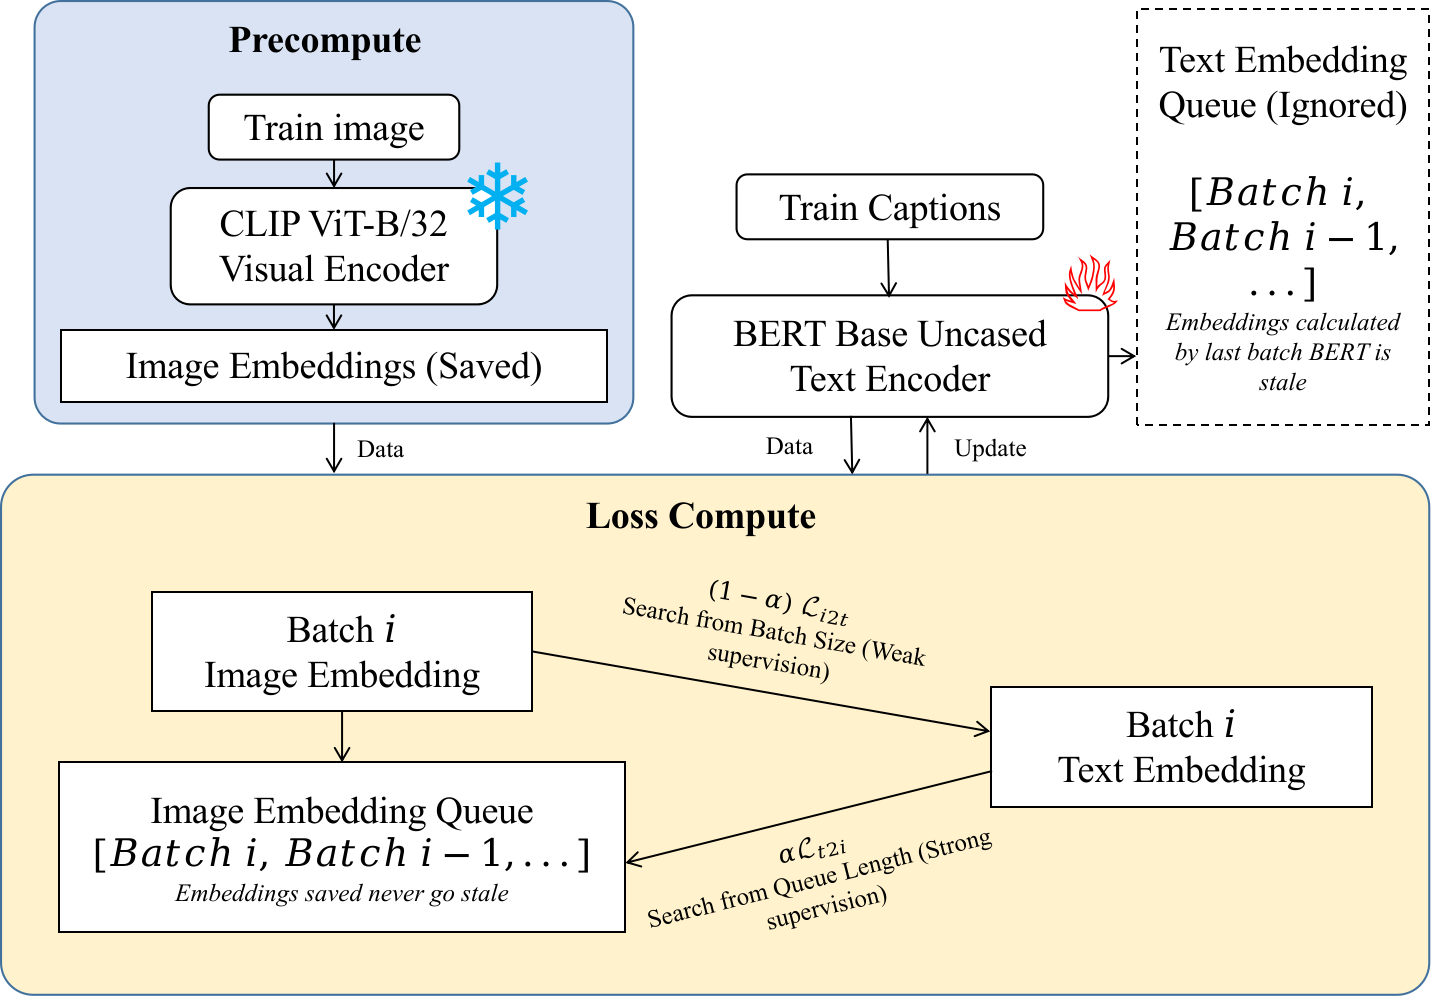
\includegraphics[width=\textwidth]{figures/Figure1.png}
\caption{Eureka-from-CLIP训练流程。冻结的CLIP视觉编码器预计算视频帧或图像嵌入（永不过时）。可训练的BERT文本编码器配合LoRA产生文本嵌入。图像队列为文本-图像学习提供丰富的负样本，而过时的文本队列则被遮蔽。}
\label{fig:pipeline}
\end{figure}

\subsection{模型架构}

模型由三个组件组成：

\textbf{冻结的CLIP视觉编码器。}我们使用OpenAI的ViT-B/32作为冻结的视觉编码器。所有图像在线下一次编码，产生512维L2归一化嵌入。

\textbf{BERT文本编码器。}我们使用BERT-base（uncased）作为文本编码器骨干网络。对于每个输入描述，从最后一层提取BERT的[CLS]令牌表示。

\textbf{投影头。}一个线性投影将768维的BERT [CLS]嵌入映射到512维共享空间，随后进行L2归一化。

\textbf{LoRA适配器（第一阶段）。}我们在BERT的query、key、value和output投影层中插入秩$r=8$、$\alpha=16$的LoRA \citep{hu2022lora}适配器。原始BERT权重保持冻结；仅LoRA参数和投影头可训练。这在110.8M总参数中产生了1.35M可训练参数。

\textbf{Stack LoRA（第二阶段）。}对于视频领域适配，我们首先使用PEFT的\texttt{merge\_and\_unload()}将训练好的r=8适配器合并到BERT权重中（即对每个目标层计算$W' = W + \frac{\alpha}{r}BA$，得到普通模型）。然后我们插入一个新的秩$r=2$、$\alpha=4$的LoRA适配器。合并后的r=8权重冻结在基础模型中；仅r=2适配器（0.63M可训练参数）参与训练。这种堆叠设计使得在最小程度遗忘原始跨模态对齐的情况下实现高效的领域迁移。

\subsection{损失函数设计}

我们采用加权非对称InfoNCE损失 \citep{oord2018representation}，公式如下：

\begin{equation}
\mathcal{L} = (1 - \alpha) \cdot \text{CE}(\mathbf{S}_{i2t} \cdot \tau, \mathbf{y}) + \alpha \cdot \text{CE}(\mathbf{S}_{t2i} \cdot \tau, \mathbf{y}),
\label{eq:asymmetric_loss}
\end{equation}

其中$\mathbf{S}_{i2t} = \mathbf{I} \mathbf{T}^{\top}$为图像-文本相似度矩阵，$\mathbf{S}_{t2i} = \mathbf{T} \mathbf{I}^{\top}$为文本-图像相似度矩阵，$\tau = \exp(\gamma)$为可学习的温度参数（初始化为$1/0.07$），$\mathbf{y}$为对角标签集（正样本对），$\text{CE}$表示交叉熵，$\alpha$为t2i权重。

我们设置$\alpha = 0.75$，给予文本-图像方向3倍于图像-文本方向的权重。这一设计选择基于实际使用场景：在文本-图像检索中，用户提供文本查询，系统检索相关图像或场景，因此文本-图像召回是更重要的指标。

\subsection{带文本过时遮蔽的队列设计}

对比学习受益于大量负样本。遵循MoCo \citep{he2020moco}，我们维护一个过去（图像、文本）嵌入对的FIFO队列。然而，一个关键挑战出现了：文本编码器正在训练，因此队列中的文本嵌入是由早期、能力较弱的模型版本产生的。这些"过时"的文本嵌入如果用作图像-文本方向的负样本，可能会提供误导性的梯度信号。

我们的核心洞察是，这种过时性是方向相关的，且这种非对称性与我们的任务目标完美对齐：

\begin{itemize}
  \item \textbf{图像-文本（i2t）：}文本队列是过时的（文本编码器在演化）。我们在该方向上完全遮蔽文本队列，仅使用批次内负样本。这实际上意味着式\ref{eq:asymmetric_loss}中的$\mathbf{S}_{i2t}$计算为$\mathbf{I}_{\text{batch}} \mathbf{T}_{\text{batch}}^{\top}$，不包含队列条目。由于t2i是我们的主要关注点，牺牲i2t的队列负样本是可接受的权衡。
  \item \textbf{文本-图像（t2i）：}图像队列\emph{不是}过时的，因为图像嵌入来自冻结的CLIP编码器。因此我们为该方向保留完整的图像队列，计算$\mathbf{S}_{t2i} = \mathbf{T}_{\text{batch}} [\mathbf{I}_{\text{batch}}; \mathbf{I}_{\text{queue}}]^{\top}$。新鲜的图像队列提供了大量且一致的负样本集，直接提升了t2i性能。
\end{itemize}

这种非对称队列设计如表\ref{tab:queue}所示。重要的是，训练哪个编码器以及保留哪一侧队列的选择并非随意。如果我们选择训练视觉编码器而冻结文本编码器，图像嵌入将变得过时，文本队列保持新鲜；此时队列将提升i2t而非t2i——与我们的需求相反。因此，我们的配置（训练文本编码器，保留图像队列）在训练目标和架构设计之间建立了自然的对齐：冻结的CLIP保证了新鲜的图像队列，新鲜的图像队列保证了强大的t2i学习。通过遮蔽过时的文本嵌入，我们进一步避免损害i2t梯度，而这又带来双重收益——因为t2i已经在损失函数中获得了更高的权重（$\alpha = 0.75$）。

\begin{table}[h]
\centering
\caption{用于文本过时感知对比学习的非对称队列设计。}
\label{tab:queue}
\begin{tabular}{c|c}
\hline
\textbf{i2t方向} & \textbf{t2i方向} \\
仅批次内负样本 & 批次内 + 队列负样本 \\
\hline
$\mathbf{I}_{\text{batch}} \mathbf{T}_{\text{batch}}^{\top}$ & $\mathbf{T}_{\text{batch}} [\mathbf{I}_{\text{batch}}; \mathbf{I}_{\text{queue}}]^{\top}$ \\
无队列（避免过时文本） & 图像队列（无过时问题） \\
\hline
\end{tabular}
\end{table}

我们额外应用了假负样本遮蔽：队列中与批次项共享相同图像ID的条目在相似度矩阵中被遮蔽（设为$-\infty$），防止它们被当作负样本处理。

\subsection{训练细节}

\textbf{第一阶段（图像对齐）：}我们在COCO train2017描述（113k图像，567k描述）上使用单张GeForce RTX 4060笔记本电脑GPU（8 GB VRAM）进行训练：
\begin{itemize}
  \item 批量大小：128（8 GB VRAM中BERT-base + LoRA可容纳的最大值）
  \item 优化器：AdamW，学习率$3\times 10^{-4}$，权重衰减0.01
  \item 调度器：线性预热（34,536步）后接余弦衰减至零
  \item 训练轮数：30
  \item 混合精度训练（AMP）
  \item 队列大小：49,152
  \item LoRA秩：8，alpha：16，dropout：0.1
\end{itemize}
队列在损失计算后更新，防止当前批次项成为自身的负样本。预计算的CLIP图像嵌入避免了冗余的视觉前向传播。整个第一阶段训练约需12小时。

\textbf{第二阶段（视频领域适配）：}我们在MSR-VTT训练描述（9k视频片段，180k描述-片段对）上使用同样的GPU：
\begin{itemize}
  \item 批量大小：128
  \item 优化器：AdamW，学习率$1\times 10^{-5}$（较低以保留对齐）
  \item 调度器：线性预热（4,000步）后接余弦衰减
  \item 训练轮数：30
  \item 混合精度训练（AMP）
  \item 队列大小：49,152
  \item Stack LoRA秩：2，alpha：4，dropout：0.1
\end{itemize}
我们在每个周期结束时在MSVD（1,970个视频，零样本）和Flickr30k（1K图像）上评估。对于视频，CLIP逐帧关键帧嵌入通过均值池化得到视频级表示。

\section{实验}

\subsection{评估设置}

我们在涵盖视频和图像检索的两个基准上进行评估：

\textbf{MSVD} \citep{chen2011collecting}是一个视频检索基准，包含来自YouTube的1,970个视频，每个视频约有20个人工标注描述。按照零样本协议，我们在标准的670视频测试集上评估，不在MSVD上进行任何训练。视频表示通过均值池化12个均匀采样的CLIP逐帧关键帧嵌入得到，遵循CLIP4Clip \citep{luo2022clip4clip}验证的简单而有效的池化策略。

\textbf{Flickr30k} \citep{plummer2015flickr30k}是一个图像检索基准，包含31,783张图像，每张有5条描述。我们使用标准的1,000张图像测试集进行零样本评估。

对于两个基准上的CLIP基线，我们使用官方OpenAI ViT-B/32模型。在视觉侧，这与我们BERT训练期间使用的冻结编码器相同。在文本侧，我们使用CLIP的原生Transformer文本编码器。

\subsection{主要结果}

表\ref{tab:video_results}展示了MSVD视频检索的主要结果。我们的两阶段方法取得了有竞争力的性能：

\begin{table}[h]
\centering
\caption{MSVD上零样本文本-视频检索结果。所有方法使用相同的冻结CLIP ViT-B/32视觉编码器，采用均值池化的帧嵌入。}
\label{tab:video_results}
\begin{tabular}{lcccccc}
\toprule
方法 & \multicolumn{3}{c}{t2i} & \multicolumn{3}{c}{i2t} \\
\cmidrule(lr){2-4} \cmidrule(lr){5-7}
 & R@1 & R@5 & R@10 & R@1 & R@5 & R@10 \\
\midrule
CLIP零样本（原生文本编码器） & 27.01 & 50.62 & 60.73 & 43.28 & 60.30 & 66.27 \\
我们的（第一阶段对齐，无视频适配） & --- & --- & --- & --- & --- & --- \\
~~+ 继续LoRA（r=8）在MSR-VTT上 & 26.95 & 54.57 & 66.35 & 44.33 & 63.73 & 70.15 \\
~~+ Stack LoRA（冻结r=8，叠加r=2） & \textbf{28.13} & \textbf{54.80} & 66.35 & \textbf{44.78} & 63.28 & \textbf{71.19} \\
\bottomrule
\end{tabular}
\end{table}

Stack LoRA配置取得了最佳的视频检索性能（28.13\% t2i R@1），超过了CLIP原生文本编码器基线（27.01\%），同时在i2t方向上也有所提升（44.78\%对比43.28\%）。相比之下，简单地在MSR-VTT上继续微调完整的r=8适配器仅获得26.95\% t2i R@1，与CLIP持平，表明没有权重合并和重新堆叠策略，模型无法有效专门化到视频领域（参见表\ref{tab:flickr_results}中对应的原始COCO对齐遗忘情况）。

表\ref{tab:flickr_results}报告了Flickr30k图像检索结果，作为视频领域适配后跨模态对齐是否保持的辅助验证：

\begin{table}[h]
\centering
\caption{Flickr30k测试集（1K图像）上的零样本图像检索结果。第一阶段结果是任何视频适配前COCO训练模型的性能。}
\label{tab:flickr_results}
\begin{tabular}{lcc}
\toprule
方法 & t2i R@1 & Flickr $\Delta$（对比第一阶段） \\
\midrule
CLIP零样本（原生文本编码器） & 57.90 & --- \\
我们的（第一阶段，COCO对齐） & \textbf{60.48} & --- \\
~~+ 继续LoRA（r=8）在MSR-VTT上 & 58.80 & $-$1.68 \\
~~+ Stack LoRA（冻结r=8，叠加r=2） & 56.90 & $-$3.58 \\
\bottomrule
\end{tabular}
\end{table}

在COCO上的第一阶段跨模态对齐产生了一个在Flickr30k上优于CLIP原生编码器的BERT文本编码器（60.48对比57.90）。通过Stack LoRA进行视频领域适配后，Flickr30k性能回落到56.90（下降了$-$3.58），这在预期之内——因为领域从COCO的静态照片转移到MSR-VTT的动态视频叙述。关键在于，这种领域偏移正是Stack LoRA所要捕捉的信号：低秩约束迫使适配器向视频领域专门化，Flickr上的退化是这种专门化的自然伴随结果，而非局限性的证据。

\subsection{分析：非对称损失和队列设计的影响}

\begin{table}[h]
\centering
\begin{tabular}{lcc}
\toprule
配置 & t2i R@1 & i2t R@1 \\
\midrule
我们的（完整） & 60.48 & 74.60 \\
无遮蔽（允许过时文本队列） & 44.32 & 53.80 \\
无队列 & 55.06 & 72.10 \\
\bottomrule
\end{tabular}
\caption{框架中各队列组件的消融实验。}
\label{tab:ablation}
\end{table}

\begin{table}[h]
\centering
\begin{tabular}{lcc}
\toprule
$\alpha$（t2i权重） & t2i R@1 & i2t R@1 \\
\midrule
0.25 & 59.28 & 76.10 \\
0.50 & 60.26 & 75.90 \\
0.75 & 60.48 & 74.60 \\
\bottomrule
\end{tabular}
\caption{非对称损失权重$\alpha$对检索性能的影响。}
\label{tab:alpha}
\end{table}

表\ref{tab:ablation}总结了消融实验。移除文本过时遮蔽（"无遮蔽"）严重降低了两个方向的性能，因为过时的文本嵌入污染了梯度。值得注意的是，这种设置比"无队列"更差，表明未遮蔽的队列对学习的危害超过没有队列。在没有队列的情况下（"无队列"），缺乏丰富的负样本主要损害了t2i。

表\ref{tab:alpha}考察了损失权重$\alpha$的影响。将$\alpha$从0.25增加到0.75仅获得了+1.20 t2i R@1的提升（从59.28到60.48），同时伴随着从i2t到t2i的相应转移。$\alpha{=}0.50$的配置达到了60.26 t2i R@1，仅比完整的$\alpha{=}0.75$设置低0.22点，表明非对称损失权重相比队列设计的贡献要小得多。

结合表\ref{tab:ablation_mlp}中的参数放置消融，这些结果建立了一个更广泛的层级：\emph{如何}将有限的可训练容量分布在BERT层之间（LoRA对比MLP，表\ref{tab:ablation_mlp}）以及\emph{如何}设计对比队列（表\ref{tab:ablation}）在决定最终检索性能方面均主导了显式的损失重加权（表\ref{tab:alpha}）。

\subsection{消融：参数分布（LoRA对比MLP投影）}

为了隔离LoRA的性能提升是源于额外的可训练容量还是其在BERT内的逐层分布，我们将所有LoRA适配器替换为一个三层MLP投影头（$768 \to 704 \to 704 \to 512$），其可训练参数数量相当（约1.40M对比LoRA配置的约1.35M）。MLP插入在BERT的[CLS]池化之后，替换了原始的线性投影头和LoRA适配器。所有其他超参数保持不变。

表\ref{tab:ablation_mlp}报告了结果。MLP投影仅达到39.92\% t2i R@1和51.3\% i2t R@1，远低于LoRA配置（60.48\% / 74.60\%），甚至低于"无队列"消融（55.06\% / 72.10\%）。t2i R@1上20多个百分点的下降表明，可训练参数的架构放置远重要于其原始数量。LoRA的有效性在于它能够适配BERT所有12个Transformer层的内部表示，而MLP将所有可训练容量集中在一个事后投影中，无法弥补冻结的BERT骨干网络与CLIP嵌入空间之间的不对齐。

有趣的是，MLP配置在早期周期后验证损失也出现平台期（val\_loss在第5个周期达到最小值2.44，之后逐渐增加），表明事后投影很快耗尽了其表示能力。相比之下，LoRA配置在整个30周期的训练过程中持续改善。

\begin{table}[h]
\centering
\caption{消融实验：LoRA对比MLP投影（可训练参数数量相当）。两种模型均在COCO上训练，在Flickr30k上进行零样本评估。}
\label{tab:ablation_mlp}
\begin{tabular}{lcccccc}
\toprule
方法 & t2i R@1 & t2i R@5 & t2i R@10 & i2t R@1 & i2t R@5 & i2t R@10 \\
\midrule
LoRA（我们的） & 60.48 & 84.96 & 91.00 & 74.60 & 92.90 & 96.60 \\
MLP投影 & 39.92 & 68.88 & 78.68 & 51.30 & 81.00 & 89.20 \\
\bottomrule
\end{tabular}
\end{table}

\section{讨论}

\subsection{队列非对称性主导检索优化}

表\ref{tab:ablation}和\ref{tab:alpha}中的消融结果揭示了设计选择之间的明确层级。完全移除队列使t2i R@1下降了5.42点（从60.48降到55.06），而将t2i权重$\alpha$从0.75降至0.50仅移动了0.22点（从60.26到60.48，表\ref{tab:alpha}）。队列带来的性能增益远大于显式损失重加权所获得的。

文本过时遮蔽更为关键：允许过时的文本嵌入进入队列（"无遮蔽"）使t2i R@1骤降至44.32，下降了16.16点。未遮蔽的队列比完全没有队列更差，表明来自过时文本嵌入的陈旧梯度不仅提供递减的收益，反而会主动损害学习。

这些结果表明，我们框架中最大的性能提升源自非对称队列机制，而非显式的损失重加权。这一洞察同样适用于视频领域，其中相同的冻结CLIP视觉编码器保证了队列中视频嵌入的新鲜度。

\subsection{为什么损失重加权不如预期重要？}

$\alpha$的相对温和影响可以通过检查训练期间的损失动态来理解。图像队列为文本-图像方向提供大量额外的负样本，使得每个批次内的t2i任务天然比i2t更困难。这种非对称性源自大型图像队列，它为t2i分支引入了数万个额外的图像负样本。因此，原始t2i损失在训练过程中始终大于对应的i2t损失。图\ref{fig:loss_ratio}绘制了整个训练轨迹中未加权的损失比$L_{t2i}/L_{i2t}$（$\alpha{=}0.75$）。值得注意的是，该比率从第一个周期的约3.3倍上升到收敛时的超过13.5倍，所有周期的均值为$11.86$倍。这一趋势违反直觉：尽管为t2i分支分配了更大的优化权重（$\alpha{=}0.75$），原始t2i损失不仅保持更高，而且在整个训练过程中与i2t的差距持续扩大。如果损失加权是主导因素，人们会预期原始t2i损失随着训练进行而趋近于i2t损失。相反，不断增长的比率表明队列引发的难度压倒了显重重加权的补偿，证实了队列非对称性——而非损失加权——是t2i优化偏差的主要驱动因素。

这一观察解释了为什么$\alpha{=}0.50$配置（表\ref{tab:alpha}）达到了60.26 t2i R@1，仅比$\alpha{=}0.75$低0.22点。队列通过非对称地向t2i提供更多负样本，作为一种隐式正则化器，降低了对显式损失加权的需求。

\begin{figure}[h]
\centering
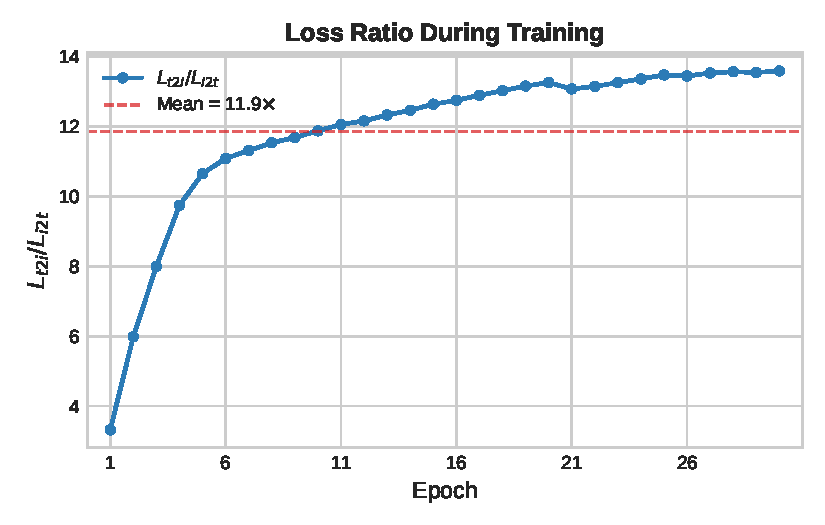
\includegraphics[width=0.72\textwidth]{figures/loss_ratio.pdf}
\caption{
\label{fig:loss_ratio}
训练期间原始（未加权）文本-图像损失与图像-文本损失的比值$L_{t2i}/L_{i2t}$（$\alpha{=}0.75$）。尽管存在偏向t2i的显式优化偏差，该比率从第一个周期的约3.3倍上升到收敛时的超过13.5倍，均值为$11.86$倍（虚线）。这一不断扩大的差距表明队列引发的非对称性主导了损失重加权的效果。
}
\end{figure}

\subsection{资源约束自然导致非对称设计}

非对称队列并非任意的设计选择。相反，它从我们资源受限的训练设置中自然产生：冻结CLIP视觉编码器使图像和视频嵌入始终保持新鲜，而演化的文本编码器则使队列中的文本嵌入过时。在这种设置下，仅保留图像队列成为最自然的解决方案。

\subsection{Stack LoRA实现高效领域迁移}

两阶段结果（表\ref{tab:video_results}、\ref{tab:flickr_results}）揭示了一个清晰的模式：Stack LoRA在视频检索上取得了强劲的性能（MSVD上28.13 t2i R@1），同时收敛速度快于全参数替代方案（25个周期对比28个周期）。相比之下，在没有权重合并和重堆叠的情况下继续微调完整的r=8适配器仅得到26.95 t2i R@1——与CLIP基线持平，比Stack LoRA低1.18点——表明权重合并和堆叠策略对于有效的领域专门化至关重要。

Stack LoRA的较小r=2适配器，由于其有限的表示容量，只能捕捉训练数据中最显著的信号——而最显著的信号恰恰就是这种图像到视频的领域偏移。低秩约束迫使适配器强烈地致力于目标领域，产生更快的收敛速度（优化器搜索空间更小）和更高的视频检索性能（每个可训练参数都专注于视频偏移）。这种专门化自然地将文本嵌入分布从COCO对齐空间向视频领域移动，这解释了观察到的Flickr退化（-$3.58$）是一种可预测的伴随结果而非局限性。

关键在于，这种可插拔性是LoRA适配的自然属性。COCO对齐的r=8适配器和MSR-VTT的r=2堆叠是独立的低秩矩阵，可以在推理时以极小的内存开销进行加载、切换或组合。当任务是图像检索时，仅需要r=8适配器；当领域转移到视频时，可以在不丢弃原始对齐的情况下将r=2堆叠插在其上。由于每个适配器只占完整模型大小的一小部分（r=8为1.35M参数，r=2为0.63M），且两者都能舒适地放在单张8\,GB GPU上，用户可以维护多个领域特定适配器并根据需要部署——这是参数高效理念的一个实际体现。

\subsection{扩展到多语言检索}

我们的框架依赖BERT作为文本编码器，这自然地扩展到多语言场景，因为BERT提供了多语言变体（如bert-base-multilingual-cased），具有跨语言的共享分词器和嵌入空间。为探索这一能力，我们在相同的英文COCO描述上使用相同的超参数训练多语言BERT，并在中文Flickr30k上进行零样本评估——其中中文描述通过HY-MT1.5 \citep{hymt152025tencent}翻译原始英文描述得到。

\begin{table}[h]
\centering
\caption{Flickr30k上的零样本多语言检索。所有模型仅使用英文COCO描述进行训练。}
\label{tab:multilingual}
\begin{tabular}{lcc}
\toprule
方法 & t2i R@1 & i2t R@1 \\
\midrule
BERT-uncased（英文，我们的） & 60.48 & 74.60 \\
多语言BERT（英文，我们的） & 57.08 & 69.00 \\
多语言BERT（中文，我们的） & 27.22 & 39.20 \\
\bottomrule
\end{tabular}
\end{table}

表\ref{tab:multilingual}报告了多语言结果。多语言BERT在英文上达到57.08\% t2i R@1，比BERT-uncased（60.48\%）低3.4点，这归因于多语言分词器对英文文本的子词效率降低。更重要的是，其在中文上达到了27.22\% t2i R@1——显著高于0.1\%的随机基线，且接近其英文性能的一半——尽管训练期间从未见过中文文本。这证明了有意义的零样本跨语言迁移：共享的多语言嵌入空间在通过仅英文的对比学习对齐到CLIP视觉表示后，能够泛化到非英文查询。

这些结果进一步说明了我们基于BERT的框架的可插拔性。由于LoRA适配器作用于BERT的内部表示而非语言特定特征，相同的英文训练适配器可以不加修改地应用于多语言BERT。在视频检索场景中，这意味着对齐到CLIP视觉空间的多语言BERT可以使用多种语言的查询检索视频，且Stack LoRA视频领域适配器随基础模型一同迁移，无需多语言视频训练数据。

\section{局限性}

我们承认本工作存在若干局限性。首先，我们的视频评估限于MSVD，这是一个相对较小的基准（1,970个视频；我们使用标准的670视频测试集）。更大且更多样化的视频检索基准如MSR-VTT 1K-A或ActivityNet将提供更全面的评估。使用简单的均值池化进行帧聚合也限制了我们捕捉视频中时序结构的能力。

其次，我们的模型仅在第一阶段使用COCO train2017描述（113k图像，567k描述）进行训练，这是一个领域多样性有限的单一数据集。虽然这使我们能够在严格的计算约束下展示方法的有效性，但在更多样化的语料库上训练可能会提高泛化能力。

第三，Flickr30k上的评估是在1K测试集上进行的，其中R@K指标的方差可能大于更大基准上的方差。

第四，消融实验报告的是无置信区间的单次运行结果。由于计算限制，每个配置仅评估一次而非使用多个随机种子，因此观察到的差异应谨慎解读。

第五，我们的多语言评估限于单一数据集（Flickr30k）上的中文，使用的是机器翻译而非人工标注的描述。HY-MT1.5 \citep{hymt152025tencent}的翻译质量可能引入噪声，低估了真正的跨语言迁移能力，在更多语言和视频基准上的评估留待未来工作。

\section{未来工作}

在此工作之外，几个方向值得探索。首先，简单的帧嵌入均值池化可以替换为更复杂的时序聚合方法，例如在帧嵌入序列上的轻量级Transformer或文本查询与视频帧之间的跨模态注意力 \citep{gorti2022xpool}。这可以更好地捕捉运动和事件结构，尤其在长视频上。

其次，在更大更多样化的视频基准（如MSR-VTT 1K-A、ActivityNet、DiDeMo）上评估将提供更全面的泛化能力评估。将框架扩展到支持多语言视频检索（即不同语言的查询从同一个视频池中检索）是我们基于BERT的方法的自然应用。

第三，探索更激进的参数效率方案（如提示调优 \citep{huang2023vop} 或稀疏适配器 \citep{cao2024acl}）可以进一步降低适配成本，而将Stack LoRA应用于其他领域迁移场景（如图像$\to$医学、英文$\to$多语言）将测试其通用性。

\section{结论}

本文介绍了Eureka-from-CLIP，一个在严格资源约束下将CLIP文本编码器替换为轻量级BERT适配器以进行零样本文本-视频检索的框架。通过两阶段方法——首先在COCO图像上将BERT对齐到CLIP的视觉空间（第一阶段），然后通过Stack LoRA进行视频领域适配（第二阶段）——我们在两个基准上取得了有竞争力的结果：Flickr30k图像检索60.48\% t2i R@1（超越CLIP的57.90\%）和MSVD视频检索28.13\% t2i R@1（优于CLIP的27.01\%），全部仅使用0.63--1.35M可训练参数，在单张8\,GB GPU上完成。

我们的文本过时感知的非对称队列设计解决了仅训练文本编码器时对比队列面临的基本挑战：通过遮蔽过时的文本嵌入同时保留新鲜的图像队列，我们防止了梯度污染并最大化丰富负样本的效益。Stack LoRA展示了冻结预训练适配器并堆叠更小的适配器可以在极小的计算开销下高效地将跨模态对齐迁移到新领域。

我们的方法为用任意BERT变体替换CLIP文本编码器提供了一种实用、可泛化的方案，使视频、多语言和领域特定检索应用无需昂贵的从头训练。

\section*{致谢}

作者感谢Jie Lei在本项目中的指导与有益讨论。本工作作为浙江工业大学Python应用开发基础课程设计完成。

\bigskip

\bibliographystyle{plainnat}
\begin{thebibliography}{99}

\bibitem[Radford et al.(2021)Radford, Kim, Hallacy, Ramesh, Goh, Agarwal, Sastry, Askell, Mishkin, Clark, Krueger, and Sutskever]{radford2021clip}
A.~Radford, J.~W.~Kim, C.~Hallacy, A.~Ramesh, G.~Goh, S.~Agarwal, G.~Sastry, A.~Askell, P.~Mishkin, J.~Clark, G.~Krueger, and I.~Sutskever.
\newblock Learning transferable visual models from natural language supervision.
\newblock In \textit{ICML}, 2021.

\bibitem[Devlin et al.(2019)Devlin, Chang, Lee, and Toutanova]{devlin2019bert}
J.~Devlin, M.-W.~Chang, K.~Lee, and K.~Toutanova.
\newblock BERT: Pre-training of deep bidirectional transformers for language understanding.
\newblock In \textit{NAACL-HLT}, 2019.

\bibitem[He et al.(2020)He, Fan, Wu, Xie, and Girshick]{he2020moco}
K.~He, H.~Fan, Y.~Wu, S.~Xie, and R.~Girshick.
\newblock Momentum contrast for unsupervised visual representation learning.
\newblock In \textit{CVPR}, 2020.

\bibitem[Hu et al.(2022)Hu, Shen, Wallis, Allen-Zhu, Li, Wang, Wang, and Chen]{hu2022lora}
E.~J.~Hu, Y.~Shen, P.~Wallis, Z.~Allen-Zhu, Y.~Li, S.~Wang, L.~Wang, and W.~Chen.
\newblock LoRA: Low-rank adaptation of large language models.
\newblock In \textit{ICLR}, 2022.

\bibitem[Chen et al.(2022)Chen, Liu, Zhang, Ye, Yang, and Wu]{chen2022altclip}
Z.~Chen, G.~Liu, B.-W.~Zhang, F.~Ye, Q.~Yang, and L.~Y.~Wu.
\newblock AltCLIP: Altering the language encoder in CLIP for extended language capabilities.
\newblock \textit{arXiv preprint arXiv:2211.06679}, 2022.

\bibitem[Yang et al.(2022)Yang, Pan, Lin, Men, Zhang, Zhou, and Zhou]{yang2022chinese}
A.~Yang, J.~Pan, J.~Lin, R.~Men, Y.~Zhang, J.~Zhou, and C.~Zhou.
\newblock Chinese CLIP: Contrastive vision-language pretraining in Chinese.
\newblock \textit{arXiv preprint arXiv:2211.01335}, 2022.

\bibitem[van den Oord et al.(2018)van den Oord, Li, and Vinyals]{oord2018representation}
A.~van den Oord, Y.~Li, and O.~Vinyals.
\newblock Representation learning with contrastive predictive coding.
\newblock \textit{arXiv preprint arXiv:1807.03748}, 2018.

\bibitem[Plummer et al.(2015)Plummer, Wang, Cervantes, Caicedo, Hockenmaier, and Lazebnik]{plummer2015flickr30k}
B.~A.~Plummer, L.~Wang, C.~M.~Cervantes, J.~C.~Caicedo, J.~Hockenmaier, and S.~Lazebnik.
\newblock Flickr30k entities: Collecting region-to-phrase correspondences for richer image-to-sentence models.
\newblock In \textit{ICCV}, 2015.

\bibitem[Lin et al.(2014)Lin, Maire, Belongie, Hays, Perona, Ramanan, Dollár, and Zitnick]{lin2014coco}
T.-Y.~Lin, M.~Maire, S.~Belongie, J.~Hays, P.~Perona, D.~Ramanan, P.~Dollár, and C.~L.~Zitnick.
\newblock Microsoft COCO: Common objects in context.
\newblock In \textit{ECCV}, 2014.

\bibitem[Conneau et al.(2020)Conneau, Khandelwal, Goyal, Chaudhary, Wenzek, Guzmán, Grave, Ott, Zettlemoyer, and Stoyanov]{conneau2020xlmr}
A.~Conneau, K.~Khandelwal, N.~Goyal, V.~Chaudhary, G.~Wenzek, F.~Guzmán, E.~Grave, M.~Ott, L.~Zettlemoyer, and V.~Stoyanov.
\newblock Unsupervised cross-lingual representation learning at scale.
\newblock In \textit{ACL}, 2020.

\bibitem[Zhai et al.(2022)Zhai, Wang, Mustafa, Steiner, Keysers, Kolesnikov, and Beyer]{zhai2022lit}
X.~Zhai, X.~Wang, B.~Mustafa, A.~Steiner, D.~Keysers, A.~Kolesnikov, and L.~Beyer.
\newblock LiT: Zero-shot transfer with locked-image text tuning.
\newblock In \textit{CVPR}, 2022.

\bibitem[Zhai et al.(2023)Zhai, Mustafa, Kolesnikov, and Beyer]{zhai2023sigmoid}
X.~Zhai, B.~Mustafa, A.~Kolesnikov, and L.~Beyer.
\newblock Sigmoid loss for language image pre-training.
\newblock In \textit{ICCV}, 2023.

\bibitem[Sharma et al.(2018)Sharma, Ding, and Soricut]{sharma2018conceptual}
P.~Sharma, N.~Ding, and R.~Soricut.
\newblock Conceptual captions: A cleaned, hypernymed, image alt-text dataset for automatic image captioning.
\newblock In \textit{ACL}, 2018.

\bibitem[Thomee et al.(2016)Thomee, Shamma, Friedland, Elizalde, Ni, Poland, Borth, and Li]{thomee2016yfcc100m}
B.~Thomee, D.~A.~Shamma, G.~Friedland, B.~Elizalde, K.~Ni, D.~Poland, B.~Borth, and L.-J.~Li.
\newblock YFCC100M: The new data in multimedia research.
\newblock \textit{Communications of the ACM}, 59(2):64--73, 2016.

\bibitem[Tencent Hunyuan Team(2025)]{hymt152025tencent}
Tencent Hunyuan Team.
\newblock HY-MT1.5 technical report.
\newblock \textit{arXiv preprint arXiv:2512.24092}, 2025.

\bibitem[Luo et al.(2022)Luo, Ji, Zhong, Chen, Lei, Duan, and Li]{luo2022clip4clip}
H.~Luo, L.~Ji, M.~Zhong, Y.~Chen, W.~Lei, N.~Duan, and T.~Li.
\newblock CLIP4Clip: An empirical study of CLIP for end to end video clip retrieval.
\newblock \textit{Neurocomputing}, 508:293--304, 2022.

\bibitem[Bain et al.(2021)Bain, Nagrani, Varol, and Zisserman]{bain2021frozen}
M.~Bain, A.~Nagrani, G.~Varol, and A.~Zisserman.
\newblock Frozen in time: A joint video and image encoder for end-to-end retrieval.
\newblock In \textit{ICCV}, 2021.

\bibitem[Lei et al.(2021)Lei, Li, Zhou, Gan, Berg, Bansal, and Liu]{lei2021clipbert}
J.~Lei, L.~Li, L.~Zhou, Z.~Gan, T.~L.~Berg, M.~Bansal, and J.~Liu.
\newblock Less is more: ClipBERT for video-and-language learning via sparse sampling.
\newblock In \textit{CVPR}, 2021.

\bibitem[Gorti et al.(2022)Gorti, Vouitsis, Ma, Golestan, Volkovs, Garg, and Yu]{gorti2022xpool}
S.~K.~Gorti, N.~Vouitsis, J.~Ma, K.~Golestan, M.~Volkovs, A.~Garg, and G.~Yu.
\newblock X-pool: Cross-modal language-video attention for text-video retrieval.
\newblock In \textit{CVPR}, 2022.

\bibitem[Huang et al.(2023)Huang, Gong, Pan, Jiang, Lv, Li, and Wang]{huang2023vop}
S.~Huang, B.~Gong, Y.~Pan, J.~Jiang, Y.~Lv, Y.~Li, and D.~Wang.
\newblock VoP: Text-video co-operative prompt tuning for cross-modal retrieval.
\newblock In \textit{CVPR}, 2023.

\bibitem[Cao et al.(2024)Cao, Tang, Huang, Jin, Zhang, Liu, Chen, Liang, Yuan, and Li]{cao2024acl}
M.~Cao, H.~Tang, J.~Huang, P.~Jin, C.~Zhang, R.~Liu, L.~Chen, X.~Liang, L.~Yuan, and G.~Li.
\newblock RAP: Efficient text-video retrieval with sparse-and-correlated adapter.
\newblock In \textit{ACL Findings}, 2024.

\bibitem[Liu et al.(2022)Liu, Xiong, Xu, Cao, and Jin]{liu2022ts2net}
Y.~Liu, P.~Xiong, L.~Xu, S.~Cao, and Q.~Jin.
\newblock TS2-Net: Token shift and selection transformer for text-video retrieval.
\newblock In \textit{ECCV}, 2022.

\bibitem[Chen and Dolan(2011)]{chen2011collecting}
D.~Chen and W.~Dolan.
\newblock Collecting highly parallel data for paraphrase evaluation.
\newblock In \textit{ACL}, 2011.

\end{thebibliography}

\section{超参数选择}

我们评估了$\alpha \in \{0.25, 0.50, 0.75\}$。尽管$\alpha{=}0.50$已经达到了可比的性能，但$\alpha{=}0.75$产生了最高的t2i R@1，因此被最终模型采用。表\ref{tab:hyperparams}总结了本框架使用的关键超参数。所有实验使用在COCO描述上训练的LoRA秩$r=8$，种子为42。

\begin{table}[h]
\centering
\caption{关键超参数。CLIP ViT-B/32（OpenAI）基线：t2i R@1~57.90\%，i2t R@1~76.90\%。}
\label{tab:hyperparams}
\begin{tabular}{lcc}
\toprule
超参数 & 值 & 描述 \\
\midrule
批量大小 & 128 & 8 GB VRAM下最大 \\
学习率 & $3\times10^{-4}$ & AdamW，余弦衰减 \\
权重衰减 & 0.01 & \\
预热步数 & 34,536 & 线性预热 \\
训练轮数 & 30 & \\
\midrule
LoRA秩 $r$ & 8 & \\
LoRA $\alpha$ & 16 & \\
LoRA dropout & 0.1 & \\
LoRA目标 & Q, K, V, O & BERT线性层 \\
\midrule
队列大小 & 49,152 & FIFO对比队列 \\
t2i权重 $\alpha$ & 0.75 & 式\ref{eq:asymmetric_loss} \\
温度 $\tau$ 初始值 & $1/0.07$ & 可学习 $\tau=\exp(\gamma)$ \\
\midrule
AMP & true & 混合精度训练 \\
\bottomrule
\end{tabular}
\end{table}

\end{document}
